\chapterimage{./Pictures/cover-inheritance}
\chapter{TP3 : Héritage et polymorphisme}
\textit{La notion d'héritage permet de réutiliser des classes. Une classe dérivée hérite des membres et méthodes d'une classe de base. L'objectif de ce TP est d'étudier les droits d'accès aux membres et méthodes d'une classe après un héritage, la construction et l'initialisation d'objets, la redéfinition de méthodes et la notion de polymorphisme. Au cours de ce TP, nous utiliserons la représentation hiérarchique des classes présentée sur le sujet.}

\section{Exercice 1 : Droits d'accès}
On remarque que la classe Personne définit les attributs nom, prenom, et age nécessaire à toutes les classes, ils ne sera donc pas nécessaire de les redéfinir dans les autres classes puisque le constructeur de la classe Personne qui est la classe mère se chargera des les initialiser. Cependant les attributs spécifique aux classes, comme l'attribut service dans la classe Personnel devront être ajoutés.\\
Chaque classe fille devra appeler le constructeur de la classe mère à l'aide du mot \textit{super} ainsi les attributs de nom, prenom et age seront correctement initialisés.\\
Les attributs définit dans la classe Personne ont des droits d'accès différents. L'attribut age est \mintinline{java}{protected}, rendant l'attribut accessible depuis les classes filles ainsi que depuis les classes du même paquet. Par contre l'attribut nom étant \mintinline{java}{private} il sera neccessaire d'utilier un accesseur et un mutateur. L'attribut prenom lui est \mintinline{java}{public} et donc accessible depuis n'importe qu'elle instance de Personne ou de ses filles. Déclaré des atrtibut \mintinline{java}{public} n'est pas conseillé on préfère généralement utiliser le mot clef \mintinline{java}{protect} ou encore les accessurs et mutateurs.\\
Les classes présentent dans ce diagramme pe uvent apparaitre en tant que classe fille mais aussi en tant que classe mere. Par exemple Personnel est à la fois une classe fille de Personne mais aussi une classe mère de Administratif et Enseignant.

\section{Exercice 1, 2 et 3 : Construction d'objets avec redéfinition de méthodes et polymorphismes}
\textit{L'objectif de cet exercice est de créer les différentes classes présentée sur le diagramme de classe, nous devons prendre en compte les informations de l'exercice précédent et utiliser les notions de redéfinition et de polymorphisme vus aux TPs précédents. Nous construirons aussi une classe Main qui instanciera les objects des classes.}
Voici le code de la classe Personne :
\inputminted[linenos,firstline=3,lastline=45]{java}{../sources/src/tp3/Personne.java}
Voici le code de la classe Personnel :
\inputminted[linenos,firstline=3,lastline=38]{java}{../sources/src/tp3/Personnel.java}
Voici le code de la classe Etudiant :
\inputminted[linenos,firstline=3,lastline=43]{java}{../sources/src/tp3/Etudiant.java}
Voici le code de la classe Administratif :
\inputminted[linenos,firstline=3,lastline=28]{java}{../sources/src/tp3/Administratif.java}
Voici le code de la classe Enseignant :
\inputminted[linenos,firstline=3,lastline=33]{java}{../sources/src/tp3/Enseignant.java}

Afin de tester le bon fonctionnement de nos implementations j'ai instancier les classes créés :
\inputminted[linenos,firstline=3,lastline=48]{java}{../sources/src/tp3/Main.java}

À l'éxecution on obtient l’affichage final suivant :
\begin{figure}[H]
  \centering
  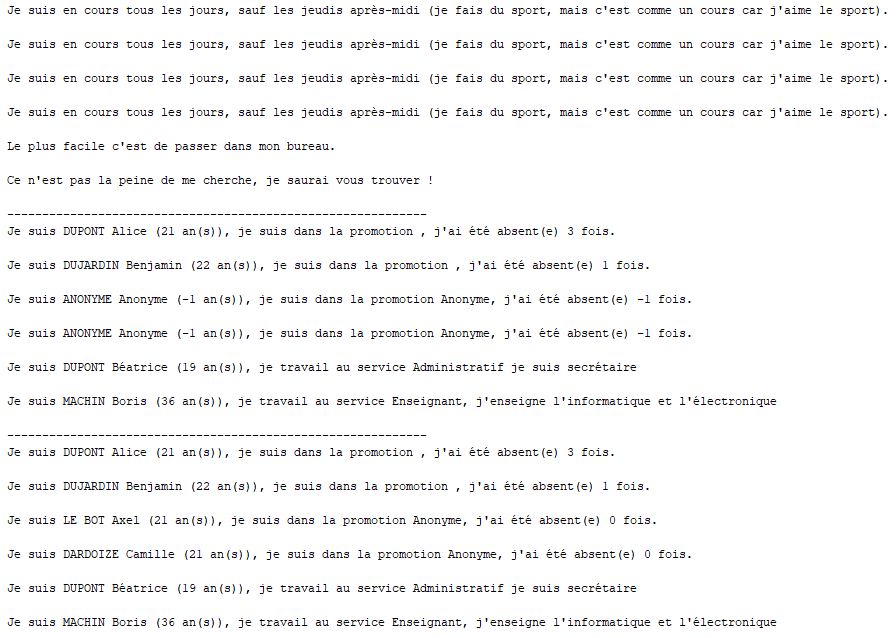
\includegraphics[width=450pt]{./tp/Pictures/tp3-execute}
  \caption{Exécution TP3}
  \label{Exécution TP3}
\end{figure}

\section{Synthèse personnelle}
Lors de ce TP nous avons bien cerné l'intérêt de l'héritage et ses conceptsonnant une meilleur compréhension et clarté du code produit. Ainsi nous nous somme familiarisé avec ces notions dans une mise en situation plus réelle.
